\documentclass [aspectratio=169]{beamer}
\beamertemplatenavigationsymbolsempty

\usepackage{textpos} % package for the positioning
\usepackage[]{graphicx}
\usepackage{graphicx}
\usepackage{float}
\usepackage{gensymb}
\usepackage{hyperref}
\usepackage{caption}
\usepackage{subcaption}
\usepackage{algorithm,algpseudocode}
\usepackage[export]{adjustbox}
\usepackage{tikz}
\usepackage[square,numbers]{natbib}
\usepackage[byname]{smartref}
\usetikzlibrary{positioning}
\usetikzlibrary{arrows, shapes, decorations, automata, backgrounds, fit, petri, calc}

% Font family and color
\newcommand*{\logofont}{\fontfamily{phv}\selectfont}
\definecolor{uwopurple}{RGB}{79,38,131}

% Title of lecture
\title[]{\texorpdfstring{\vspace{60pt} \\ 
Functionalities, Performance, Pricings \\ 
Choosing the text editor of your choice}}

% set color
\setbeamercolor{title in head/foot}{bg=white}
\setbeamercolor{author in head/foot}{bg=white}
\setbeamercolor{date in head/foot}{fg=uwopurple}
\setbeamercolor{date in head/foot}{bg=white}
\setbeamercolor{title}{fg=uwopurple}
\setbeamerfont{title}{series=\bfseries}
\setbeamercolor{frametitle}{fg=uwopurple}
\setbeamerfont{frametitle}{series=\bfseries}
\setbeamercolor{block title}{bg=uwopurple!30,fg=black}
\setbeamercolor{item}{fg=uwopurple}
\setbeamercolor{caption name}{fg=uwopurple!70!}

\begin{document}

\date{}

{
\begin{frame}
    \titlepage
    \begin{textblock*}{8cm}(5.0cm,-7.0cm)
        \huge \color{uwopurple}{\textbf{Text Editor}}
    \end{textblock*}
\end{frame}
}

{
\begin{frame}{1.0 What is a text editor}
    \begin{itemize}
        \item Simply put, a text editor is a software that allows you to write, update and delete text from a file.
        \item Remember, code are basically just text, but when we refer to something as a text editor, most of the time we imply that it is used for writing code.
        \item Some text editors you might know is: \textbf{Visual Studio}, \textbf{NetBeans}, \textbf{Emacs}, \textbf{Vim}, \textbf{Neovim}...
        \item Google Docs can also be considered as a text editor, but when referring to it as a text editor, we do not mean it is made to handle code.
    \end{itemize}
\end{frame}
}

{
\begin{frame}{2.0 Why do we need a text editor}
    \begin{itemize}
        \item When coding, we often rely on syntax highlighting and auto completion to help us with distinguish between different types of objects as well as auto complete long
        function or variable names. 
        \item A text editor will allow you to accomplish these goals by connecting itself with a tree sitter for syntax highlighting and an LSP for autocompletion.
        \item Syntax highlighting in Visual Studio Code:
            {
                \centering
                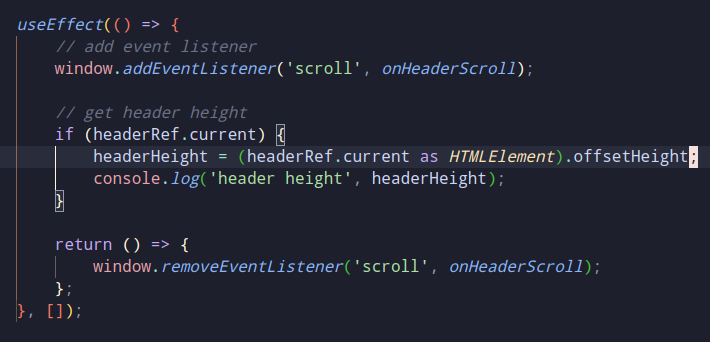
\includegraphics[width=0.5\linewidth]{figures/vscode-treesitter.png}
            }
    \end{itemize}
\end{frame}
}
{
\begin{frame}{3.0 Text editor vs IDE}
    \begin{itemize}
        \item Actually, I lied to your earlier. The syntax highlighting and autocompletion technically isn't part of a text editor. When a text editor has these features, it transform into an IDE.
        \item An IDE (Integrated Development Environment) is a software specifically made to write code and has features that supports writing code.
        \item So in that sense, the image of Visual Studio Code earlier is actually an image of an IDE, but because modern IDEs offer much more than just syntax highlighting and code completion, we rarely refer to VS Code as an IDE but rather as a text editor.
        \item Modern IDEs such as PyCharm, IntelliJ... offer syntax highlighting, autocompletion, debugging capabilities, snippets for specific languages and anything else you might need. These functions are \textbf{integrated} into a single software for you to use.
    \end{itemize}
\end{frame}
}
{
\begin{frame}{4.0 Choosing a text editor / IDE}
    \begin{itemize}
        \item When choosing a text editor or an IDE, it all comes down to preferences.
        \item \textbf{Choose an IDE} if you want a software that is ready right out of the box for you to use instantly. When using an IDE, you will also be exposed to many functionalities that might be beneficial to speed up your development process. The \textbf{downside} of an IDE is that they are often cumbersome and resource intensive. Most of the good IDEs now are also paid products or offer a free tier vs paid tier such as PyCharm, IntelliJ...
        \item \textbf{Choose a text editor} if you want a lightweight software to edit code with minimal functionalities (or at least minimal out of the box). Text editors often offer a large range of configurations and customizations, but because they are quite barren out of the box, this requires the user to put in the effort to make them to work.
    \end{itemize}
\end{frame}
}

{
\begin{frame}{5.0 My personal choice}
    \begin{itemize}
        \item \textbf{My personal choice}: I personally went with a text editor, mainly because I want something that is lightweight (because my laptop sucks) and offer many configuration options. After deciding that I want a text editor, I went with \textbf{Neovim} as the editor of my choice. Here is a screen shot of me using Neovim to write this presentation:
            {
                \centering
                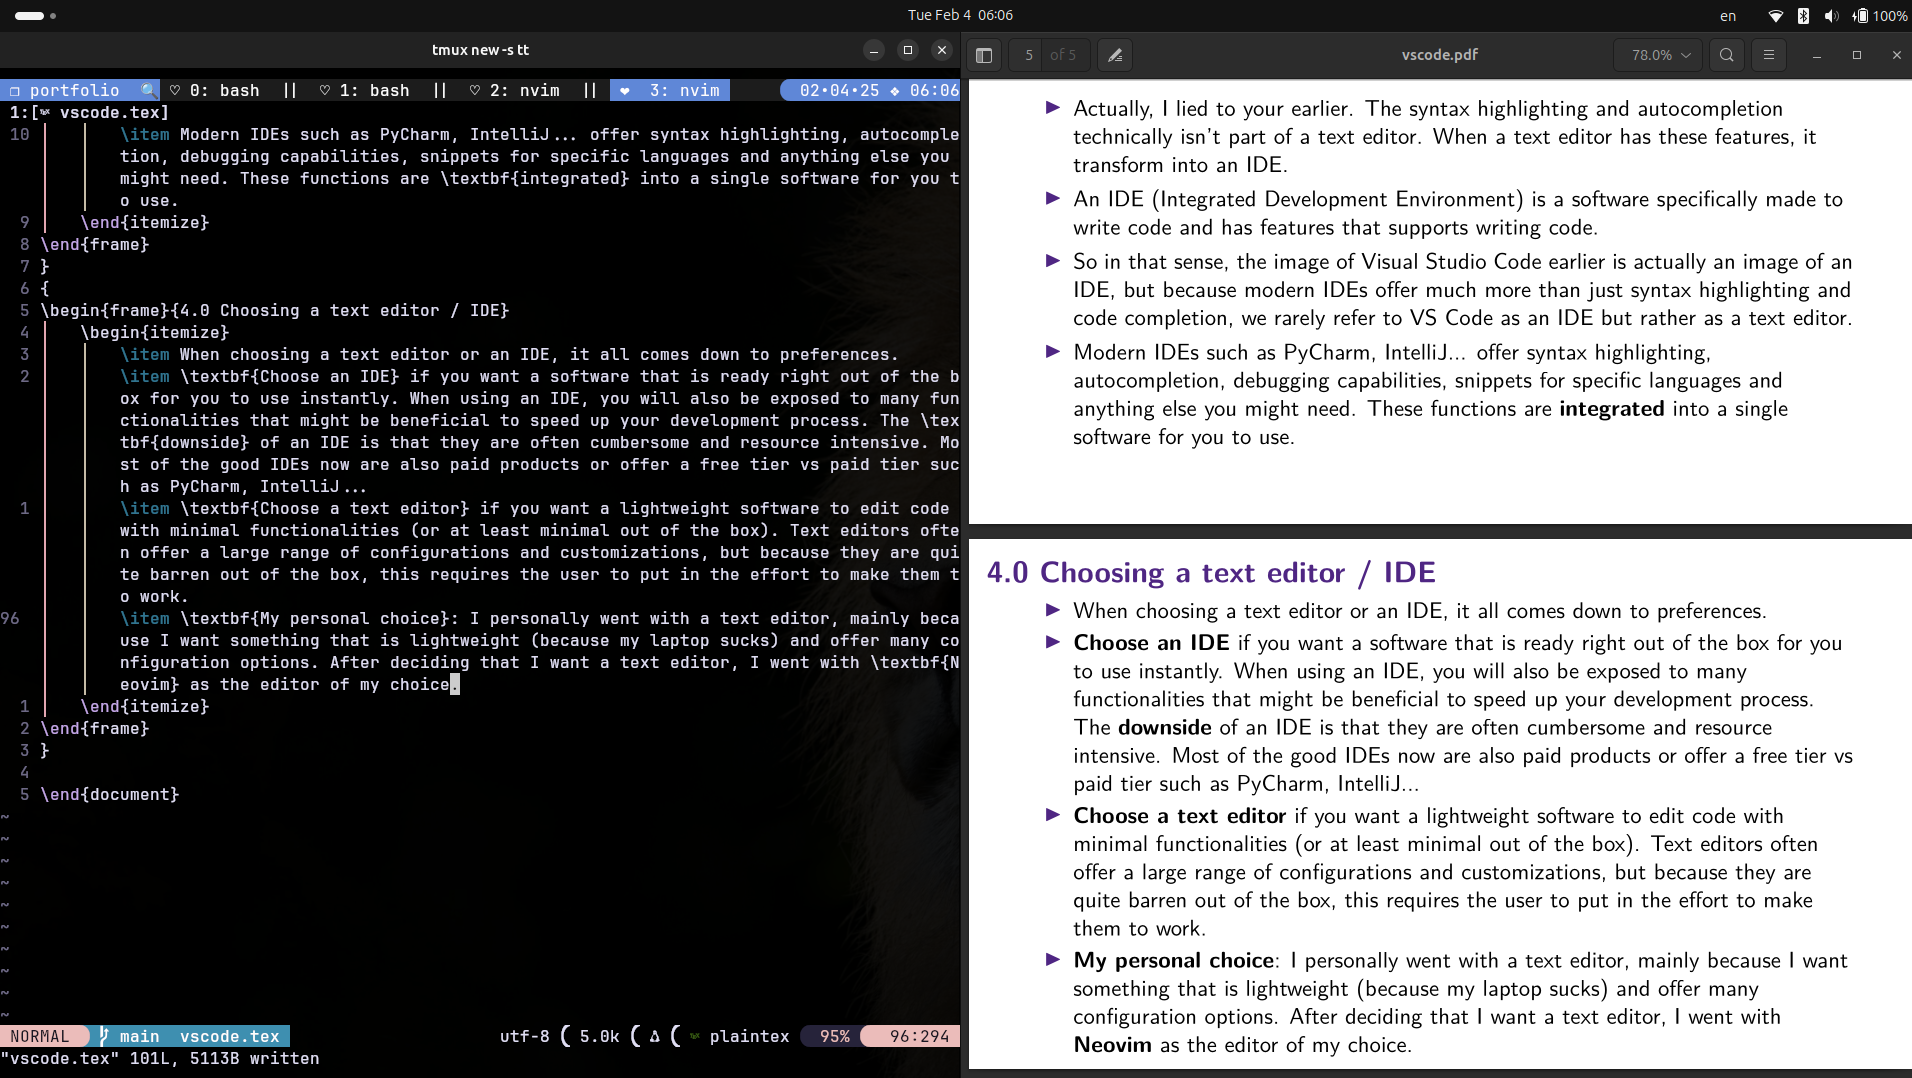
\includegraphics[width=0.5\linewidth]{figures/neovim.png}
            }
    \end{itemize}
\end{frame}
}
{
\begin{frame}{6.0 A good text editor to start out}
    \begin{itemize}
        \item If you are unsure with what you want or want to try out a good default option, I recommend \textbf{Microsoft Visual Studio Code}.
        \item Visual Studio Code is a text editor but also offers a lot of functionalities thorugh its massive \textbf{plugins ecosystem} that you can install with a few mouse clicks.
        \item VS Code is also quite simple to use and is open source so it is constantly getting updates that improves its performance and capacity. 
        \item The downside of VS Code I have oberved after many years of using it is that in large projects, it is slow and can be \textbf{very} memory intensive. It can also be slow in very large files such as large text files when dealing with machine learning or data science.
    \end{itemize}
\end{frame}
}
{
\begin{frame}{7.0 A final note}
    \begin{itemize}
        \item Whichever editor you use, your development speed and quality ultimately comes down to your ability to understand logic and write good code.
        \item So if you don't want to think too much about text editors, go with VS Code and spend time learning how to write good code instead. 
        \item Please don't spend hours and hours configuring your text editor (\textit{like me}) if you want to save time.
    \end{itemize}
\end{frame}
}

\end{document}
